%!TEX program = xelatex
\documentclass[12pt]{article}

% ---------- IDIOMA Y FUENTE ----------
\usepackage{fontspec} 
\usepackage[spanish, es-tabla, es-nodecimaldot]{babel} 
% --- Cambiar "Cuadro" por "Tabla" ---
\addto\captionsspanish{\renewcommand{\tablename}{Tabla}}
\setmainfont{TeX Gyre Termes}

% ---------- PAQUETES MATEMÁTICOS Y FÍSICOS ----------
\usepackage{amsmath,amssymb,amsfonts}
\usepackage{physics}

% ---------- GRÁFICOS Y COLORES ----------
\usepackage{xcolor}
\usepackage{graphicx}
\usepackage{tikz}
\usetikzlibrary{babel} 
\usepackage{tikz-3dplot}
\usetikzlibrary{shapes, arrows, positioning}
\usetikzlibrary{arrows.meta, angles, quotes, calc, patterns} 
\usetikzlibrary{shapes.geometric} 
\usetikzlibrary{decorations.markings}

% ---------- CÓDIGO (LISTINGS) ----------
\usepackage{listings}
\definecolor{codegreen}{rgb}{0,0.6,0}
\definecolor{codegray}{rgb}{0.95,0.95,0.95}
\definecolor{codepurple}{rgb}{0.58,0,0.82}
\definecolor{backcolour}{rgb}{0.96,0.96,0.96}

\lstdefinestyle{pythonstyle}{
    backgroundcolor=\color{backcolour},   
    commentstyle=\color{codegreen},
    keywordstyle=\color{magenta},
    numberstyle=\tiny\color{gray},
    stringstyle=\color{codepurple},
    basicstyle=\ttfamily\small,          
    breakatwhitespace=false,         
    breaklines=true,                     
    captionpos=b,                    
    keepspaces=true,                 
    numbers=left,                        
    numbersep=5pt,                  
    showspaces=false,                
    showstringspaces=false,
    showtabs=false,                  
    tabsize=4,
    language=Python                      
}
\lstset{style=pythonstyle}

% ---------- DISEÑO Y ESTILO ----------
\usepackage{geometry}
\geometry{letterpaper, margin=2cm, headheight=15pt}
\usepackage{fancyhdr} 
\usepackage{lastpage}
\usepackage{wrapfig}
\usepackage{multicol}
\usepackage{enumitem}
\usepackage{framed}
\usepackage{etoolbox}
\usepackage{tabularx}

% ---------- TCOLORBOX ----------
\usepackage[most,skins,theorems]{tcolorbox}

% --- Caja para Definiciones Formales ---
\newtcolorbox{definicion}[1][]{
  enhanced,
  breakable, 
  colback=blue!5!white,
  colframe=blue!75!black,
  fonttitle=\bfseries,
  title={Definición: #1},
  arc=2mm,
  boxrule=0.8pt,
  drop shadow=black!10!white
}

% --- Caja para Tareas ---
\newtcolorbox{problemas}[1][]{
  enhanced,
  breakable, 
  colback=violet!6!white,       
  colframe=violet!45!white,     
  coltitle=violet!40!black,     
  fonttitle=\bfseries,
  title={Problemas: #1},
  arc=2.5mm,                    
  boxrule=0.8pt,
  drop shadow=black!8!white     
}

% --- Caja Libre Verde Menta ---
\newtcolorbox{cajaflex}[1][]{
  enhanced,
  breakable, 
  colback=teal!5!white,       
  colframe=teal!50!black,     
  coltitle=teal!10!white,     
  fonttitle=\bfseries,
  code={\ifblank{#1}{}{\tcbset{title={#1}}}},
  arc=2.5mm,                  
  boxrule=0.8pt,
  drop shadow=black!8!white   
}

% ---------- TABLAS Y ELEMENTOS EXTRA ----------
\usepackage{booktabs}   
\usepackage{pifont}     
\usepackage{array}      
\usepackage{caption}    
\newcommand{\lapiz}{\ding{46}\ }

% ---------- CONFIGURACIÓN DE ENCABEZADOS (ITM) ----------
\newcommand{\logo}{
\includegraphics[height=3cm]{escudoitm}}
\newcommand{\escola}{Facultad de Ciencias Exactas y Aplicadas}
\newcommand{\disc}{Física Computacional 1}
\newcommand{\auth}{Robinson Longas Bedoya}
\newcommand{\emaill}{\url{robinsonlongas@itm.edu.co}}
\newcommand{\email}{\url{robinsonlongas3586@correo.itm.edu.co}}
\newcommand{\cabec}{Física Computacional 1}

% ---------- ENLACES Y PDF ----------
\usepackage{hyperref}

\definecolor{myblue}{RGB}{20, 20, 120}
\definecolor{myred}{RGB}{220, 30, 30}
\definecolor{mygreen}{RGB}{0, 130, 60}

% Personalización de nombres para \autoref
\def\tableautorefname{Tabla}
\def\figureautorefname{Figura}
\def\equationautorefname{Ecuación}
\def\sectionautorefname{Sección}

\hypersetup{
    colorlinks=true,
    linkcolor=blue,
    urlcolor=blue,
    citecolor=blue,
    pdftitle={Física Computacional 1 -- Robinson Longas Bedoya},
    pdfauthor={Robinson Longas Bedoya}
}

% Configuración de estilos de página
\pagestyle{fancy}
\fancyhf{} 

\fancypagestyle{firstpage}{
    \fancyhead[L]{\logo}
    \fancyhead[R]{
        \textsf{\escola \\} 
        \textsf{\disc \\}
        \textsf{\auth \\}
        \textsf{\email \\} 
        \textsf{\emaill}     
    }
    \fancyfoot[R]{\scriptsize Página \thepage~de \pageref{LastPage}}
    \renewcommand{\headrulewidth}{0pt} 
    \renewcommand{\footrulewidth}{0.4pt} 
}

\fancyhead[L]{\textsf{\scriptsize \cabec\ -- \auth\ -- \email\ -- \emaill}}
\fancyfoot[R]{\scriptsize Página \thepage~de \pageref{LastPage}}
\renewcommand{\headrulewidth}{0.4pt} 
\renewcommand{\footrulewidth}{0.4pt} 

\setlength{\parskip}{0.3em}

\begin{document}
		\thispagestyle{firstpage}
		\vspace*{1.5cm}
	
	\begin{center}
		\rule{\textwidth}{0.4pt}
	\end{center}
	
	\begin{itemize}[leftmargin=*,label=\textcolor{red}{\ensuremath{\blacktriangleright}}]
		\item \textbf{Números aleatorios}
	\end{itemize}
	
	\noindent
	\textbf{\underline{Bibliografía}}
	\begin{itemize}[leftmargin=*, label={\textcolor{blue}{$\bullet$}}]
		\item \textit{Computational Physics}, Mark Newman.
        \item \textit{Programming for computations - Python}, Evein Linge and Petter Langtangen. 
        \item \textit{Computational Physics with Python}, Eric Ayars. 
        \item \textit{Computational mathematics: An introduction to 
        Numerical Analysis and Scientific Computing  with Python}, Dimitrios Mitsotakis. 
        \item \textit{Computational physics: problem solving with Python}, 
        Rubin H. Landau, Manuel J. Páez and Cristian C. Bordeianu.
    \end{itemize}
     
    

\section*{\textcolor{red}{\textit{Generador de congruencia lineal}}}

Si nos piden que digamos números al azar, comenzamos a nombrar los primeros que se nos vengan a la cabeza: 
tal vez los que más nos gusten, tal vez solo positivos, tal vez números primos... La pregunta es: 
¿en realidad son al azar? Supongamos que mejor se los pedimos al computador. ¿Resolvería esto el problema? 
Recordemos que el computador solo conoce ceros y unos: opera de forma estrictamente determinista y, en rigor, 
no puede generar azar verdadero. 

\textit{Decimos que una secuencia de números $x_0, x_1, \dots, x_n$ es aleatoria si no existe una correlación estadística entre ellos}. 
A lo máximo que podemos aspirar con arquitecturas deterministas es a la generación de números \textbf{pseudoaleatorios}. 

El método clásico por excelencia es el \textbf{Generador de Congruencia Lineal (GCL)}: fijamos una semilla $x_0$ 
y, a partir de ella, generamos los términos sucesivos mediante la relación de recurrencia:
\begin{equation*}
    x_{n+1} = (a x_n + c) \pmod m.
\end{equation*}
La elección adecuada de los parámetros $a$ (multiplicador), $c$ (incremento) y $m$ (módulo) determina la calidad y el período del generador.

\begin{cajaflex}[\texttt{Ejemplo}]
Tomemos $a=5$, $c=3$ con módulo $m=8$. A partir de la semilla $x_0=1$, el GCL genera sucesivamente:
\begin{equation*}
    0,\, 3,\, 2,\, 5,\, 4,\, 7,\, 6,\, 1,\, 0,\, 3,\, \dots
\end{equation*}
Observamos que recorre todos los residuos posibles módulo 8 antes de volver a la semilla inicial $x_0=1$, completando un período de longitud $P = 8$.
\end{cajaflex}

En la siguiente tabla se muestran los valores utilizados usualmente 
para los parámetros $a, c, m$.
%
\begin{table}[htbp]
\centering
\small
\caption{Parámetros de generadores lineales clásicos frente a generadores modernos.}
\label{tab:prng_parametros}
\begin{tabular}{lcccc}
\hline
\textbf{Sistema / Implementación} & \textbf{Tipo} & $a$ & $c$ & $m$ \\
\hline
IBM RANDU (System/360)   & LCG & $65\,539$ & $0$ & $2^{31}$ \\
ANSI C (\texttt{rand} MSVC) & LCG & $214\,013$ & $2\,531\,011$ & $2^{32}$ \\
POSIX \texttt{drand48}   & LCG & $25\,214\,903\,917$ & $11$ & $2^{48}$ \\
Numerical Recipes (32-bit)& LCG & $1\,664\,525$ & $1\,013\,904\,223$ & $2^{32}$ \\
Java \texttt{Random}     & LCG & $25\,214\,903\,917$ & $11$ & $2^{48}$ \\
\hline
NumPy (\texttt{default\_rng}) & PCG64 & $6\,364\,136\,223\,846\,793\,005$ & Dinámico (128-bit) & $2^{128}$ \\
\hline
\end{tabular}
\end{table}
%

\begin{itemize}
    \item \textbf{IBM RANDU (década de 1960):} Fue el generador estándar instalado en las computadoras centrales (mainframes) IBM System/360. Diseñado en una época donde los ciclos de CPU eran carísimos, sus parámetros se eligieron para que la multiplicación se pudiera calcular con operaciones binarias ultrarrápidas (\textit{shifts} y sumas). Es recordado como el peor generador ampliamente utilizado en la historia de la computación científica.
    
    \item \textbf{ANSI C (\texttt{rand}):} Es la función de aleatoriedad básica que venía por defecto en los compiladores estándar del lenguaje C (como Microsoft Visual C++ o Turbo C). Es un LCG de 32 bits elemental y bastante pobre para física computacional.
    
    \item \textbf{POSIX \texttt{drand48}:} La rutina estándar de los sistemas operativos UNIX y distribuciones Linux para generar números en coma flotante de doble precisión. Al usar 48 bits en lugar de 32, ofreció una mejora notable para la época.
    
    \item \textbf{Numerical Recipes (Press et al.):} Es la famosa ``biblia'' del cómputo científico. Sus autores propusieron valores específicos para $a, c, m$ calculados cuidadosamente para maximizar el período en 32 bits ($m = 2^{32}$) sin sufrir las fallas evidentes de RANDU.
    
    \item \textbf{Mersenne Twister (MT19937) / NumPy Legacy:} Durante casi 20 años fue el rey indiscutible de la computación científica y el motor por defecto en \texttt{np.random.RandomState}, Python estándar (\texttt{random}), MATLAB y R. No es un LCG; funciona con matrices lineales y registros de desplazamiento sobre campos finitos. Su período es astronómico ($2^{19937} - 1$, un primo de Mersenne), pero consume mucha memoria de estado (unos 2.5 kilobytes) y falla pruebas estadísticas modernas muy rigurosas.
    
    \item \textbf{PCG64 (\texttt{np.random.default\_rng}):} Significa \textit{Permuted Congruential Generator} de 64 bits. Es el estándar moderno de NumPy desde la versión 1.17. Es una idea brillante: por debajo utiliza un LCG gigantesco de 128 bits para el estado interno, pero \textbf{nunca entrega el número tal cual}. Aplica una función no lineal de mezcla y rotación de bits a la salida (\textit{output permutation}). Esto destruye cualquier patrón reticular o alineación geométrica, siendo rapidísimo, consumiendo poquísima memoria y superando todas las baterías de pruebas estadísticas actuales.
\end{itemize}

A continuación se muestra la generación de números aleatorios 
construyendo el GLC a mano y usando el generador de \texttt{NumPy}
%
\begin{lstlisting}[language=Python, captionpos=t, title=\texttt{numeros\_aleatorios.py}]
import numpy as np
import matplotlib.pyplot as plt

def lcg(size, seed=23):
    """Genera un arreglo de N número entre (0,1) usando xn+1 = axn + c mod m"""
    a = 1103515245 
    c = 12345
    m = 2**31

    numeros = np.empty(size)
    x0 = seed
    xn = x0
    
    for i in range(size):
        xn = (a*xn + c) % m
        numeros[i] = xn/m
    return numeros

if __name__== "__main__":

    N = 10000 
    semilla = 12

    #datos a mano con Linear congruence
    datos_lcg = lcg(N,semilla) * 1000

    # datos con numpy 
    rng = np.random.default_rng(seed=semilla) # instanciamos semilla
    datos_numpy = rng.random(N) * 1000

    # 3. Scatter Plots 
    fig, axes = plt.subplots(1, 2, figsize=(11, 5))

    # Scatter LCG (A mano)
    axes[0].scatter(datos_lcg[:-1], datos_lcg[1:], s=1, color='crimson', alpha=0.5)
    axes[0].set_title("Correlación $x_n$ vs $x_{n+1}$ (A mano - LCG)", fontweight='bold')
    axes[0].set_xlabel("$x_n$")
    axes[0].set_ylabel("$x_{n+1}$")

    # Scatter NumPy
    axes[1].scatter(datos_numpy[:-1], datos_numpy[1:], s=1, color='teal', alpha=0.5)
    axes[1].set_title("Correlación $x_n$ vs $x_{n+1}$ (NumPy - PCG64)", fontweight='bold')
    axes[1].set_xlabel("$x_n$")
    axes[1].set_ylabel("$x_{n+1}$")

    plt.tight_layout()

    plt.savefig("../Clases/Herramientas_Python/random.pdf", bbox_inches='tight')
    plt.show()
\end{lstlisting}
%
\begin{figure}[htbp]
    \centering
    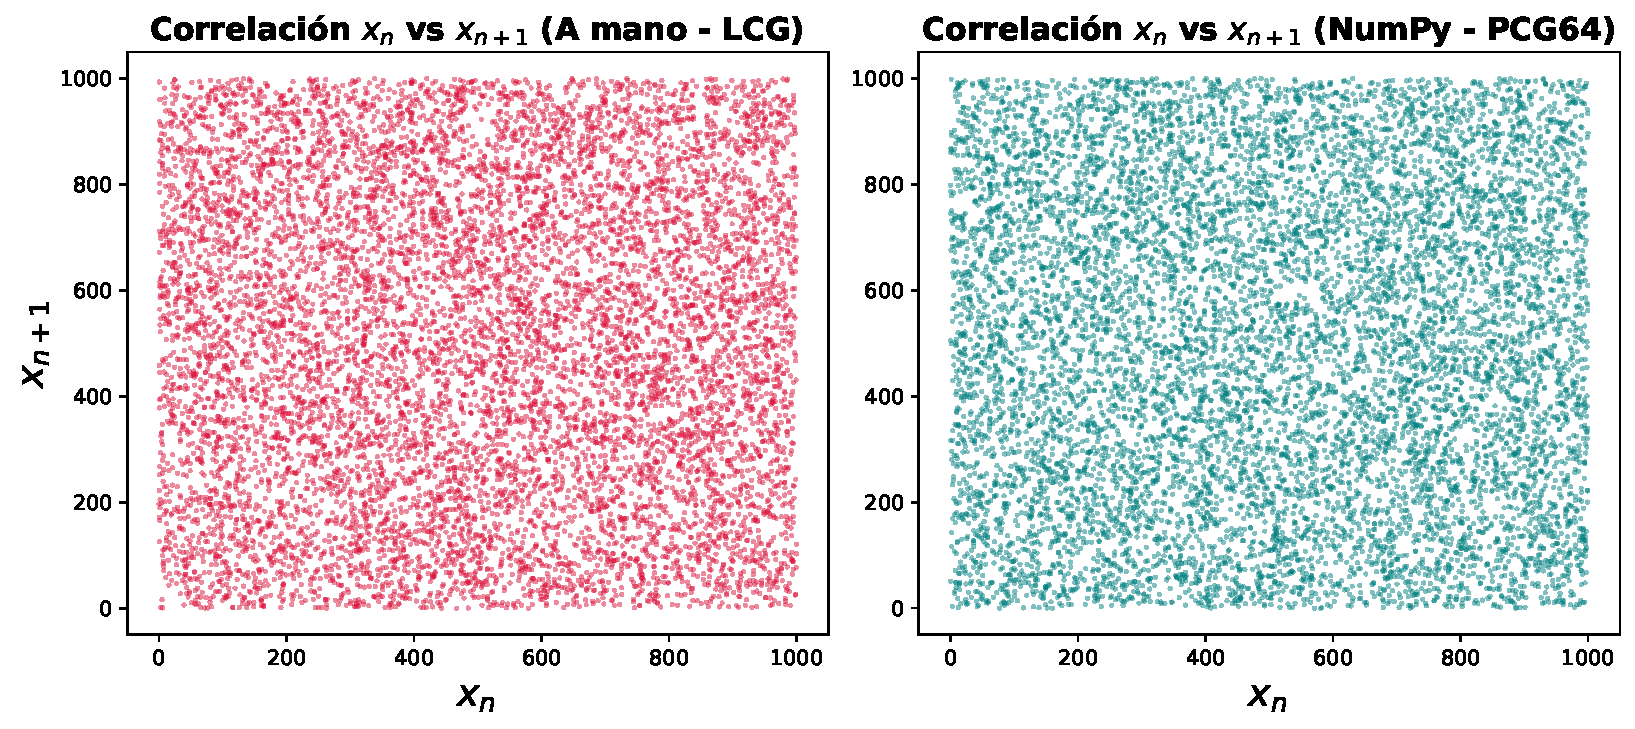
\includegraphics[width=0.8\textwidth]{random.pdf}
    \caption{Generación de números aleatotios.}
\end{figure}
%

Desde la versión 1.17, \texttt{NumPy} separó por completo el 
problema de los números aleatorios en dos capas independientes:
\begin{enumerate}
    \item \textbf{BitGenerators (El motor de bits en bruto):} Rutinas de bajo nivel escritas en C cuyo único trabajo es generar secuencias de enteros de 32 o 64 bits pseudoaleatorios a máxima velocidad.
    \item \textbf{Generators (Las distribuciones estadísticas):} La interfaz de usuario creada con \texttt{default\_rng()}, la cual toma los bits suministrados por el \textit{BitGenerator} y los transforma analíticamente en variables continuas o discretas (Uniforme, Gaussiana, Poisson, Exponencial, etc.).
\end{enumerate}

\begin{figure}[htbp]
\centering
\texttt{[ Semilla (Seed) ]} $\longrightarrow$ \textbf{\texttt{BitGenerator (PCG64)}} $\xrightarrow{\text{bits crudos}}$ \textbf{\texttt{Generator (default\_rng)}} $\longrightarrow$ \texttt{Arreglos de datos}
\caption{Esquema de dos capas del módulo \texttt{numpy.random}.}
\label{fig:numpy_random_arch}
\end{figure}

Aunque \texttt{np.random.default\_rng()} utiliza \textbf{PCG64} por defecto, \texttt{NumPy} incluye cuatro motores intercambiables según el tipo de simulación:

\begin{itemize}
    \item \textbf{\texttt{PCG64} (Estándar recomendado):} 
    Es un \textit{Permuted Congruential Generator} de 64 bits. Internamente mantiene un estado de 128 bits governado por un LCG y un incremento impar variable. Sin embargo, no entrega los bits del LCG directamente: aplica una función de permutación no lineal sobre el estado para truncar y rotar los bits salientes. Combina excelente velocidad, poquísimo uso de memoria caché y aprueba las pruebas estadísticas más exigentes del estándar \textit{BigCrush}.
    
    \item \textbf{\texttt{PCG64DXSM} (Recomendado para cómputo paralelo masivo):} 
    Una variante de PCG que introduce una permutación multiplicativa más agresiva (\textit{DXSM: Double-xorshift-multiply}). Se diseñó para evitar pequeños defectos de correlación que pueden surgir cuando se bifurcan millones de flujos aleatorios (\textit{streams}) en clústeres paralelos o múltiples hilos.
    
    \item \textbf{\texttt{MT19937} (Mersenne Twister):} 
    El motor clásico basado en matrices de torsión sobre campos de Galois $\mathbb{F}_2$. Posee un período de $2^{19937} - 1$, pero consume un estado grande de 2.5\,KB por instancia y es un 30--50\% más lento que PCG64. Se mantiene principalmente para reproducir código histórico o comparar simulaciones previas a 2019.
    
    \item \textbf{\texttt{Philox} y \texttt{SFC64} (Criptográficos y computación GPU/HPC):}
    \begin{itemize}
        \item \textbf{\texttt{Philox}} es un generador basado en cifrado por bloques (\textit{counter-based}). Es ideal para GPUs y paralelismo masivo distribuido, ya que permite calcular el estado $n$-ésimo de la secuencia de forma directa en $\mathcal{O}(1)$ sin iterar los pasos previos.
        \item \textbf{\texttt{SFC64}} (\textit{Small Fast Chaotic}): Basado en autómatas caóticos de 256 bits, es el generador más veloz en CPU, pasando también todas las pruebas estadísticas estándar.
    \end{itemize}
\end{itemize}

\subsection*{\textcolor{magenta}{\textit{Las distribuciones más utilizadas en física computacional}}} 

\begin{table}[htbp]
\centering
\small
\caption{Una vez instanciado el generador con \texttt{rng = np.random.default\_rng(semilla)}, los métodos disponibles para generar datos son:}
\label{tab:numpy_distribuciones}
\begin{tabularx}{\textwidth}{l p{4.2cm} X}
\hline
\textbf{Método} & \textbf{Distribución / Operación} & \textbf{Aplicación física típica} \\
\hline
\texttt{rng.random(size)} & Uniforme continua $U \in [0.0, 1.0)$ & Algoritmos de Monte Carlo, ruletas \\
\texttt{rng.uniform(low, high, size)} & Uniforme continua en $[a, b)$ & Posiciones iniciales homogéneas \\
\texttt{10**rng.uniform(a, b, size)} & Escala logarítmica continua $[10^a, 10^b]$ & Barridos de parámetros (acoplamientos, masas) \\
\texttt{rng.lognormal(mean, sigma, size)} & Lognormal $\ln(X) \sim \mathcal{N}(\mu, \sigma)$ & Tamaños de grano, turbulencia, astrofísica \\
\texttt{rng.logseries(p, size)} & Serie logarítmica discreta & Distribución de especies, percolación \\
\texttt{rng.integers(low, high, size)} & Enteros equiprobables en $[a, b)$ & Espines en modelo de Ising, pasos discretos \\
\texttt{rng.normal(loc, scale, size)} & Gaussiana $\mathcal{N}(\mu, \sigma)$ & Velocidades de Maxwell-Boltzmann, ruido térmico \\
\texttt{rng.exponential(scale, size)} & Exponencial $\lambda e^{-\lambda t}$ & Decaimiento radiactivo, caminos libres medios \\
\texttt{rng.poisson(lam, size)} & Conteo de Poisson & Conteo de fotones en detectores, eventos raros \\
\texttt{rng.choice(a, size, replace, p)} & Muestreo discreto ponderado & Cadenas de Markov (Metropolis-Hastings) \\
\hline
\end{tabularx}
\end{table}

\begin{cajaflex}[\texttt{Dato curioso curioso: el desastre de RANDU y el Teorema de Marsaglia}]
El generador de IBM, RANDU, utilizaba los parámetros:
\begin{align*}
    x_{n+1} = 65539 \, x_n \pmod{2^{31}}, \quad \text{con } c = 0.
\end{align*}

El valor $a = 65539$ no fue fruto del rigor estadístico, sino de la pereza del hardware: en base 2, $65539 = 2^{16} + 3$. Esto permitía a los programadores calcular la multiplicación $a \cdot x_n$ simplemente desplazando bits a la izquierda 16 posiciones ($x_n \ll 16$) y sumándole $x_n + 2x_n$, evitando la costosa instrucción de multiplicación en el procesador.

El costo científico fue catastrófico. En 1968, el matemático George Marsaglia publicó un célebre artículo titulado \textit{Random Numbers Fall Mainly in the Planes} (Los números aleatorios caen principalmente en los planos), demostrando que cualquier generador congruencial lineal sufre de regularidades reticulares. 

En el caso específico de RANDU, si tomamos tres números consecutivos $x_n, x_{n+1}, x_{n+2}$:
\begin{align*}
    x_{n+2} &= (2^{16} + 3) x_{n+1} \pmod{2^{31}} \\
            &= (2^{16} + 3)^2 x_n \pmod{2^{31}} \\
            &= (2^{32} + 6 \cdot 2^{16} + 9) x_n \pmod{2^{31}}.
\end{align*}
Dado que $2^{32} \equiv 0 \pmod{2^{31}}$, y manipulando algebraicamente los términos con $x_{n+1} = (2^{16} + 3) x_n$, se deduce la relación lineal exacta:
\begin{align*}
    x_{n+2} - 6 x_{n+1} + 9 x_n \equiv 0 \pmod{2^{31}}.
\end{align*}

Si graficamos ternas de puntos consecutivos $(x_n, x_{n+1}, x_{n+2})$ en el 
espacio tridimensional $\mathbb{R}^3$, en lugar de llenar homogéneamente el cubo 
unitario como esperaríamos de un gas o un medio aleatorio, 
\textbf{todos los puntos se concentran exclusivamente sobre apenas 15 planos 
bidimensionales paralelos}.
Décadas de simulaciones de Monte Carlo en física nuclear, termodinámica y 
astrofísica realizadas en los años 60 y 70 tuvieron que ser descartadas o 
recalculadas porque los resultados reflejaban la geometría de estos 15 
planos y no la física del problema.
\end{cajaflex}


\subsection*{\textcolor{blue}{\textit{Ejemplo: Estimación del valor de $\pi$}}} 

%
\begin{figure}[htbp]
    \centering
    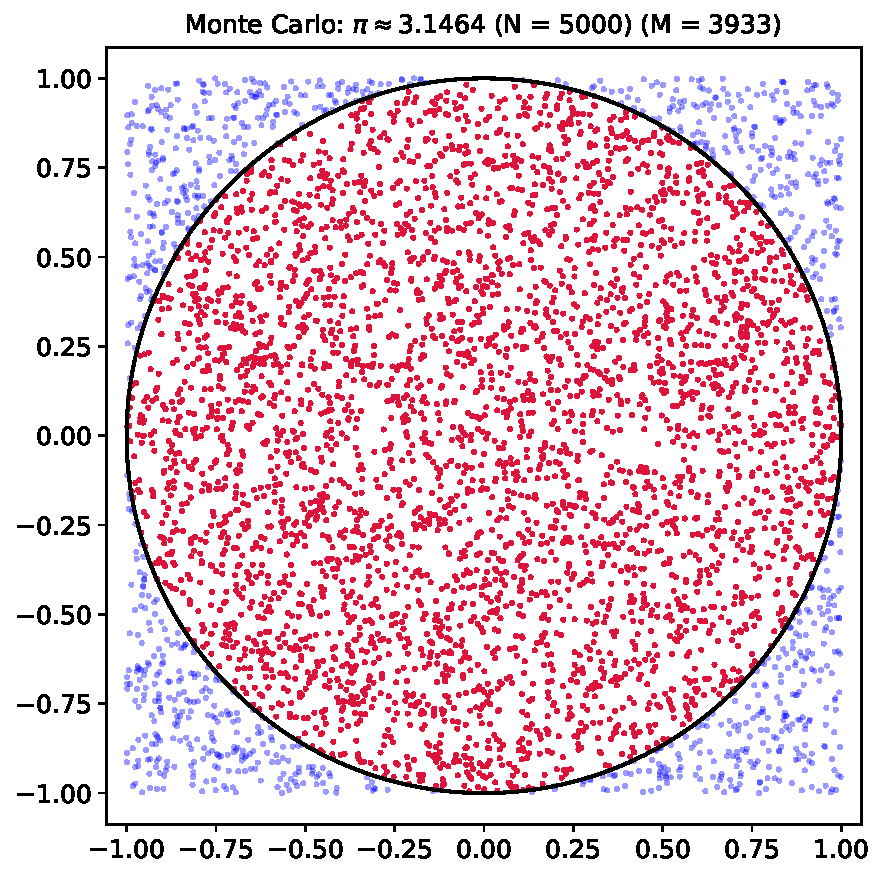
\includegraphics[width=0.4\textwidth]{pirandom.pdf}
    \caption{Estimación de $\pi$ usando números aleatorios.}
\end{figure}
%

Una de las aplicaciones simples de los números aleatorios
es el cáculo de $\pi$.
Imagina que inscribimos un círculo de radio $R$  
centrado en el origen en un cuadrado de lado $L = 2R $,
delimitado por $[-R, R] \times [-R, R]$. Tomememos por 
comodidad $R = 1$ u. Sabemos que el 
área del cuadrado $A_{\square} = L\times L = (2R)^2 = 4$ $u^2$.
Por otro lado, el área del círculo inscrito es:
$A_{\bigcirc} = \pi R^2 = \pi$ $u^2$.

Suponga entonces que generamos N puntos aleatorios 
en rectángulo $[-1, 1] \times [-1, 1]$. 
De estos puntos, claramente no todos van a caer dentro 
del círculo.  Digamos que unos M caen en el interior del 
círculo. Entonces,  $\dfrac{A_{\bigcirc}}{A_{\square}} = \dfrac{M}{N}$
 es la probabilidad de que un punto aleatorio caiga dentro del
 círculo. Luego, $\pi = 4 \dfrac{M}{N} $. Es decir, solo 
 tenemos que contar el número de puntos que caen en en el interior 
 del círculo y dividirlos por los totales, entonces si división
 es proporcional a $\pi$. 

\begin{lstlisting}[language=Python, captionpos=t, title=\texttt{pi\_random.py}]
iimport matplotlib.pyplot as plt
import numpy as np


def monte_carlo_pi(N=5000, seed=42):
  rng = np.random.default_rng(seed)
  x = rng.uniform(-1, 1, N)
  y = rng.uniform(-1, 1, N)
  adentro = x**2 + y**2 <= 1.0 # se define el disco de radio 1
  M = np.sum(adentro) # suma todos los puntos adentro del círculo
  pi_ran = 4.0 * M / N
  return x, y, adentro, pi_ran, M


if __name__ == "__main__":
  N = 5000
  x, y, adentro, pi_aprox, M = monte_carlo_pi(N)

  plt.figure(figsize=(6, 6), facecolor='white')
  plt.scatter(x[adentro], y[adentro], s=2, color="crimson")
  plt.scatter(x[~adentro], y[~adentro], s=2, color="blue", alpha=0.4)

  # Frontera
  theta = np.linspace(0, 2 * np.pi, 200)
  plt.plot(np.cos(theta), np.sin(theta), "k-", lw=1.5)

  plt.axis("equal")
  plt.xlim(-1.05, 1.05)
  plt.ylim(-1.05, 1.05)
  plt.title(f"Monte Carlo: $\\pi \\approx {pi_aprox:.4f}$ (N = {N}) (M = {M})")
  plt.tick_params (axis='both', which='both', labelsize =12)
  plt.tight_layout()
  plt.savefig('../Clases/Herramientas_Python/pirandom.pdf', bbox_inches='tight')

  plt.show()
\end{lstlisting}
%  


\subsection*{\textcolor{blue}{\textit{Ejemplo 2: camino de una persona borracha en 1D}}} 

Imaginemos a una persona caminante sobre una línea recta unidimensional que 
parte del origen $x_0 = 0$ en el instante $t = 0$. En cada intervalo de tiempo 
discreto $\Delta t = 1$ s, esta persona da un paso de longitud fija $\ell = 1$ m:
\begin{itemize}
    \item Hacia la derecha ($+1$) con probabilidad $1/2$.
    \item Hacia la izquierda ($-1$) con probabilidad $q = 1 - 1/2 = 1/2$.
\end{itemize}


Definimos el $i$-ésimo paso como una variable aleatoria discreta $s_i \in \{-1, +1\}$ tal que:
\begin{equation}
    P(s_i = +1) = \frac{1}{2}, \quad P(s_i = -1) = \frac{1}{2}.
\end{equation}
Las propiedades estadísticas de un paso individual son inmediatas:
\begin{align}
    \langle s_i \rangle &= (+1)\left(\frac{1}{2}\right) + (-1)\left(\frac{1}{2}\right) = 0, \\
    \langle s_i^2 \rangle &= (+1)^2\left(\frac{1}{2}\right) + (-1)^2\left(\frac{1}{2}\right) = 1, \\
    \text{Var}(s_i) &= \langle s_i^2 \rangle - \langle s_i \rangle^2 = 1.
\end{align}

La posición de la persona después de dar $N$ pasos sucesivos es la suma de los 
pasos individuales:
\begin{equation}
    X_N = \sum_{i=1}^N s_i.
\end{equation}

\paragraph{Valor esperado (Desplazamiento medio):}
Por linealidad del valor esperado:
\begin{equation}
    \langle X_N \rangle = \left\langle \sum_{i=1}^N s_i \right\rangle = \sum_{i=1}^N \langle s_i \rangle = 0.
\end{equation}
En promedio, el caminante nunca se aleja del punto de partida.

\paragraph{Desplazamiento Cuadrático Medio:}
Para cuantificar cuánto se dispersa típicamente del origen, calculamos $\langle X_N^2 \rangle$:
\begin{equation}
    X_N^2 = \left( \sum_{i=1}^N s_i \right)\left( \sum_{j=1}^N s_j \right) = \sum_{i=1}^N s_i^2 + \sum_{i \neq j} s_i s_j.
\end{equation}
Tomando el promedio estadístico (ensamble) y recordando que los pasos son estadísticamente independientes ($\langle s_i s_j \rangle = \langle s_i \rangle \langle s_j \rangle = 0$ para $i \neq j$):
\begin{equation}
    \langle X_N^2 \rangle = \sum_{i=1}^N \langle s_i^2 \rangle + \sum_{i \neq j} \langle s_i s_j \rangle = \sum_{i=1}^N 1 + 0 = N.
\end{equation}

\begin{cajaflex}[\texttt{La ley de difusión $\sqrt{N}$}]
La distancia típica que se recorre respecto al origen (la desviación estándar o raíz del desplazamiento cuadrático medio, RMS) escala como la raíz cuadrada del número de pasos:
\begin{equation}
    x_{\text{rms}} = \sqrt{\langle X_N^2 \rangle} = \sqrt{N}.
\end{equation}
Si el número de pasos es proporcional al tiempo ($N \propto t$), encontramos la 
rúbrica fundamental del transporte difusivo: la distancia típica crece como 
$\sqrt{t}$, en contraste con el transporte balístico determinista donde la distancia crece como $t$.
\end{cajaflex}

\begin{lstlisting}[language=Python, captionpos=t, title=\texttt{drunk\_walk.py}]
import math
import random
import matplotlib.pyplot as plt
import numpy as np


def drunk_1d(N, L=1.0):
    """
    Simula caminantx aleatorio en 1D.
    Paso Δx ~ [-L, L].
    """
    x = 0.0 #centrado en 0
    x_history = [x]

    for _ in range(N): #note que no uso el contador i porque no lo necesito
        x += (random.random() - 0.5) * 2.0 * L # paso aleatorio entre -1 y 1
        x_history.append(x)

    return x_history


def drunk_2d(N, L=1.0):
    """
    Simula caminantx aleatorio en 2D.
    Pasos independientes Δx, Δy ~ [-L, L].
    """
    x, y = 0.0, 0.0
    x_history, y_history = [x], [y]

    for _ in range(N):
        x += (random.random() - 0.5) * 2.0 * L
        y += (random.random() - 0.5) * 2.0 * L
        x_history.append(x)
        y_history.append(y)

    return x_history, y_history

def drunk_3d(N, L=1.0):
    """
    Simula caminantx aleatorio en 3D.
    Pasos independientes Δx, Δy, Δz ~ [-L, L].
    """
    x, y, z = 0.0, 0.0, 0.0
    x_history, y_history, z_history = [x], [y], [z]

    for _ in range(N):
        x += (random.random() - 0.5) * 2.0 * L
        y += (random.random() - 0.5) * 2.0 * L
        z += (random.random() - 0.5) * 2.0 * L
        x_history.append(x)
        y_history.append(y)
        z_history.append(z)

    return x_history, y_history, z_history 


if __name__ == "__main__":

    # ---------------------------------------------------------
    # PARÁMETROS GENERALES
    # ---------------------------------------------------------
    N = 1000  # Número total de pasos
    L = 10.0
    n_pasos = list(range(N + 1))
    semilla =42

    random.seed(semilla) 
    np.random.seed(semilla)

    # 1D
    x_1d = drunk_1d(N, L=L)
    x_final_1d = x_1d[-1]
    
    # 2D
    x_2d, y_2d = drunk_2d(N, L=L)
    x_final_2d, y_final_2d = x_2d[-1], y_2d[-1]
    
    # 3D
    x_3d, y_3d, z_3d = drunk_3d(N, L=L)
    x_final_3d, y_final_3d, z_final_3d = x_3d[-1], y_3d[-1], z_3d[-1]
    
    # ---------------------------------------------------------
    # PLOTS 
    # ---------------------------------------------------------
    fig = plt.figure(figsize=(18, 5))

    # --- Subplot 1: Random Walk 1D (x vs Tiempo/Pasos) ---
    ax1 = fig.add_subplot(1, 3, 1)
    ax1.plot(n_pasos, x_1d, color='royalblue', linewidth=1.5, label='Trayectoria $x(N)$')
    ax1.plot(0, x_1d[0], 'go', markersize=7, label='Inicio')
    ax1.plot(N, x_final_1d, 'ro', markersize=7, label='Fin')

    ax1.set_title('Random Walk 1D', fontweight='bold')
    ax1.set_xlabel('Número de pasos ($N$)')
    ax1.set_ylabel('Posición $x$')
    ax1.grid(True, linestyle='--', alpha=0.5)
    ax1.legend(loc='upper left', fontsize=9)

    # --- Subplot 2: Random Walk 2D (Plano X-Y) ---
    ax2 = fig.add_subplot(1, 3, 2)
    ax2.plot(x_2d, y_2d, color='royalblue', linewidth=1, alpha=0.85, label='Trayectoria')
    ax2.plot(0, 0, 'go', markersize=8, label='Inicio (0,0)')
    ax2.plot(x_final_2d, y_final_2d, 'ro', markersize=8, label='Fin')

    ax2.set_title('Random Walk 2D', fontweight='bold')
    ax2.set_xlabel('Posición $x$')
    ax2.set_ylabel('Posición $y$')
    ax2.set_aspect('equal', 'datalim')
    ax2.grid(True, linestyle='--', alpha=0.5)
    ax2.legend(loc='upper right', fontsize=9)

    # --- Subplot 3D: Espacio X-Y-Z ---
    ax3 = fig.add_subplot(1, 3, 3, projection='3d')
    ax3.plot(x_3d, y_3d, z_3d, color='royalblue', linewidth=1, alpha=0.85, label='Trayectoria')
    ax3.plot([0], [0], [0], 'go', markersize=7, label='Inicio (0,0,0)')
    ax3.plot([x_3d[-1]], [y_3d[-1]], [z_3d[-1]], 'ro', markersize=7, label='Fin')

    ax3.set_title('Random Walk 3D', fontweight='bold')
    ax3.set_xlabel('Posición $x$')
    ax3.set_ylabel('Posición $y$')
    ax3.set_zlabel('Posición $z$')
    ax3.legend(loc='upper right', fontsize=8)

    fig.tight_layout()
    plt.savefig('../Clases/Herramientas_Python/drunk.pdf', bbox_inches='tight')
    plt.show()
\end{lstlisting}
%  

%
\begin{figure}[htbp]
    \centering
    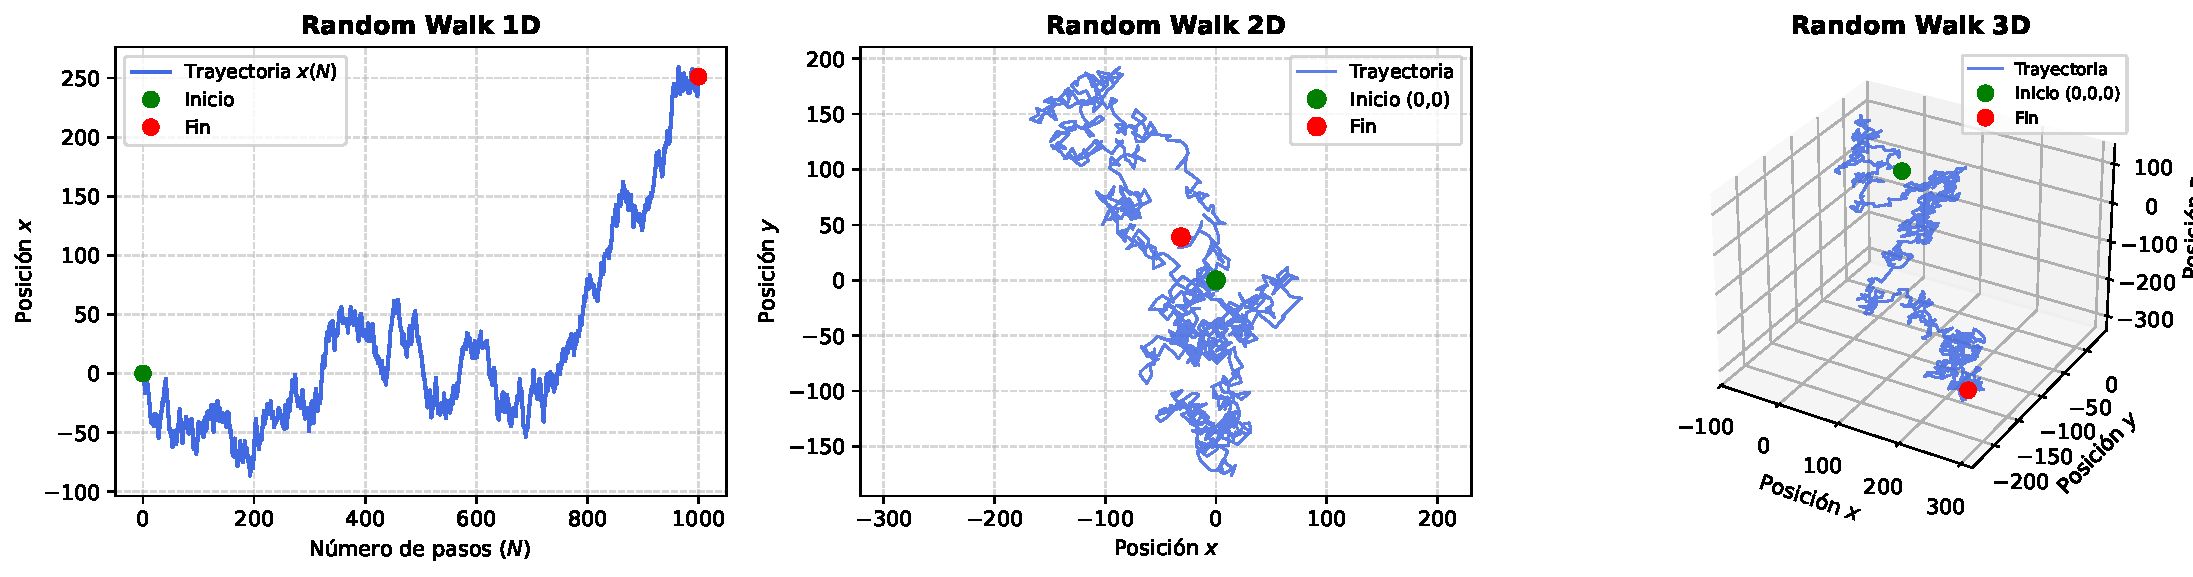
\includegraphics[width=0.95\textwidth]{drunk.pdf}
    \caption{Random walk.}
\end{figure}
%

En el código \lstinline|animation_drunk.py| puede encontrar la animación para dos 
y tres dimensiones.

\begin{lstlisting}[language=Python, captionpos=t, title=\texttt{julia\_mandelbroot.py}]
import matplotlib.pyplot as plt
import numpy as np


def mandelbrot(xmin=-2.0, xmax=0.5, ymin=-1.25, ymax=1.25, width=1000, height=1000, max_iter=200):
  """Calcula la matriz para el Conjunto de Mandelbrot.
  Mantiene z0 = 0 y varía c.
  
  Parámetros:

  xmin, xmax: rango para el eje horizopntal. parte real de c
  ymin, ymax = rango para el eje vertical. parte imaginaria de c
  width, height: resolución de la imagen (por defecto $1000 \times 1000 = 10^6$ puntos).
  max_iter: El límite de iteraciones por punto. Si desíés de 200 pasos |z|<2 se asume que 
  pertenece al conjunto de Mandelbrot.

  Devuelve:

  escape_grid: Una matriz 2D de enteros de tamaño (height, width). Cada celda (i, j) 
  almacena el número de iteraciones en las que ese punto escapó 
  (un valor entre $0$ y $199$), o $200$ (max_iter) si el punto nunca escapó y 
  se quedó atrapado dentro del fractal.

  (xmin, xmax, ymin, ymax): Una tupla con las coordenadas extremas. 
  Estas se usan para graficar con plt.imshow y graficar los valores físicos en lugar del 
  índice de píxeles del arreglo.
  """

  x = np.linspace(xmin, xmax, width)
  y = np.linspace(ymin, ymax, height)
  C = x + 1j * y[:, None]  # Matriz de parámetros c La coma crea una segunda dimensión en el array
  Z = np.zeros_like(C, dtype=np.complex128) # se crea la martriz de ceros con la dimensión de C
  escape_grid = np.full(C.shape, max_iter, dtype=int) # matriz para enviar a imshow

  # Máscara para rastrear los puntos con |z| <= 2 
  mask = np.ones(C.shape, dtype=bool)

  for i in range(max_iter):
    Z[mask] = Z[mask] ** 2 + C[mask] #aplicamos la ecuación z = z**2 +c para la mascara true
    escaped = np.abs(Z) > 2.0 # True si no pertenecen al conjunto, False si sí pertenece
    newly_escaped = escaped & mask
    escape_grid[newly_escaped] = i
    mask &= ~escaped # los puntos que quedan, se niegan los que no estan
    if not np.any(mask):
      break

  return escape_grid, (xmin, xmax, ymin, ymax)


def julia(c, xmin=-1.5, xmax=1.5, ymin=-1.5, ymax=1.5, width=1000, height=1000, max_iter=200):
  """Calcula la matriz para un Conjunto de Julia fijado en c.
  Mantiene c constante y varía las condiciones iniciales z0.

  Parámetros:
  
   xmin, xmax: rango para el eje horizopntal. parte real de c
   ymin, ymax = rango para el eje vertical. parte imaginaria de c
   width, height: resolución de la imagen (por defecto $1000 \times 1000 = 10^6$ puntos).
   max_iter: El límite de iteraciones por punto. Si desíés de 200 pasos |z|<2 se asume que 
   pertenece al conjunto de Mandelbrot.
  
  Devuelve:
  escape_grid: Una matriz 2D de enteros de tamaño (height, width). Cada celda (i, j) 
  almacena el número de iteraciones en las que ese punto escapó 
  (un valor entre $0$ y $199$), o $200$ (max_iter) si el punto nunca escapó y 
  se quedó atrapado dentro del fractal.
  (xmin, xmax, ymin, ymax): Una tupla con las coordenadas extremas. 
  Estas se usan para graficar con plt.imshow y graficar los valores físicos en lugar del 
  índice de píxeles del arreglo.
   """
  
  x = np.linspace(xmin, xmax, width)
  y = np.linspace(ymin, ymax, height)
  Z = x + 1j * y[:, None]  # Matriz de condiciones iniciales z0
  escape_grid = np.full(Z.shape, max_iter, dtype=int)

  mask = np.ones(Z.shape, dtype=bool)

  for i in range(max_iter):
    Z[mask] = Z[mask] ** 2 + c
    escaped = np.abs(Z) > 2.0
    newly_escaped = escaped & mask
    escape_grid[newly_escaped] = i
    mask &= ~escaped
    if not np.any(mask):
      break

  return escape_grid, (xmin, xmax, ymin, ymax)

if __name__ == "__main__":
  
  #c_interesante = -0.7 + 0.27015j
  #c_interesante = -0.75 + 0.0j
  #c_interesante = 0.285 + 0.01j
  c_interesante = -0.8 + 0.156j
  # Genera matrices numéricas
  grid_mandelbrot, ext_m = mandelbrot(max_iter=300)
  grid_julia, ext_j = julia(c=c_interesante, max_iter=300)

  # plot
  fig, (ax1, ax2) = plt.subplots(1, 2, figsize=(14, 6), facecolor="black")

  # Mandelbrot Plot
  ax1.imshow(grid_mandelbrot, extent=ext_m, cmap="twilight_shifted", origin="lower" )
  ax1.set_title("Conjunto de Mandelbrot", color="white", fontsize=11,fontweight="bold")
  ax1.set_xlabel("Re(c)", color="white")
  ax1.set_ylabel("Im(c)", color="white")
  ax1.tick_params(colors="white")

  # Julia Plot
  ax2.imshow(grid_julia, extent=ext_j, cmap="twilight_shifted", origin="lower")
  ax2.set_title( f"Conjunto de Julia para $c = {c_interesante}$", color="white", fontsize=11,fontweight="bold")
  ax2.set_xlabel("Re($z_0$)", color="white")
  ax2.set_ylabel("Im($z_0$)", color="white")
  ax2.tick_params(colors="white")

  plt.tight_layout()
  plt.savefig('../Clases/Herramientas_Python/julia_manderboot.pdf', bbox_inches='tight')
  plt.show()
\end{lstlisting}
%  
%
\begin{figure}[htbp]
    \centering
    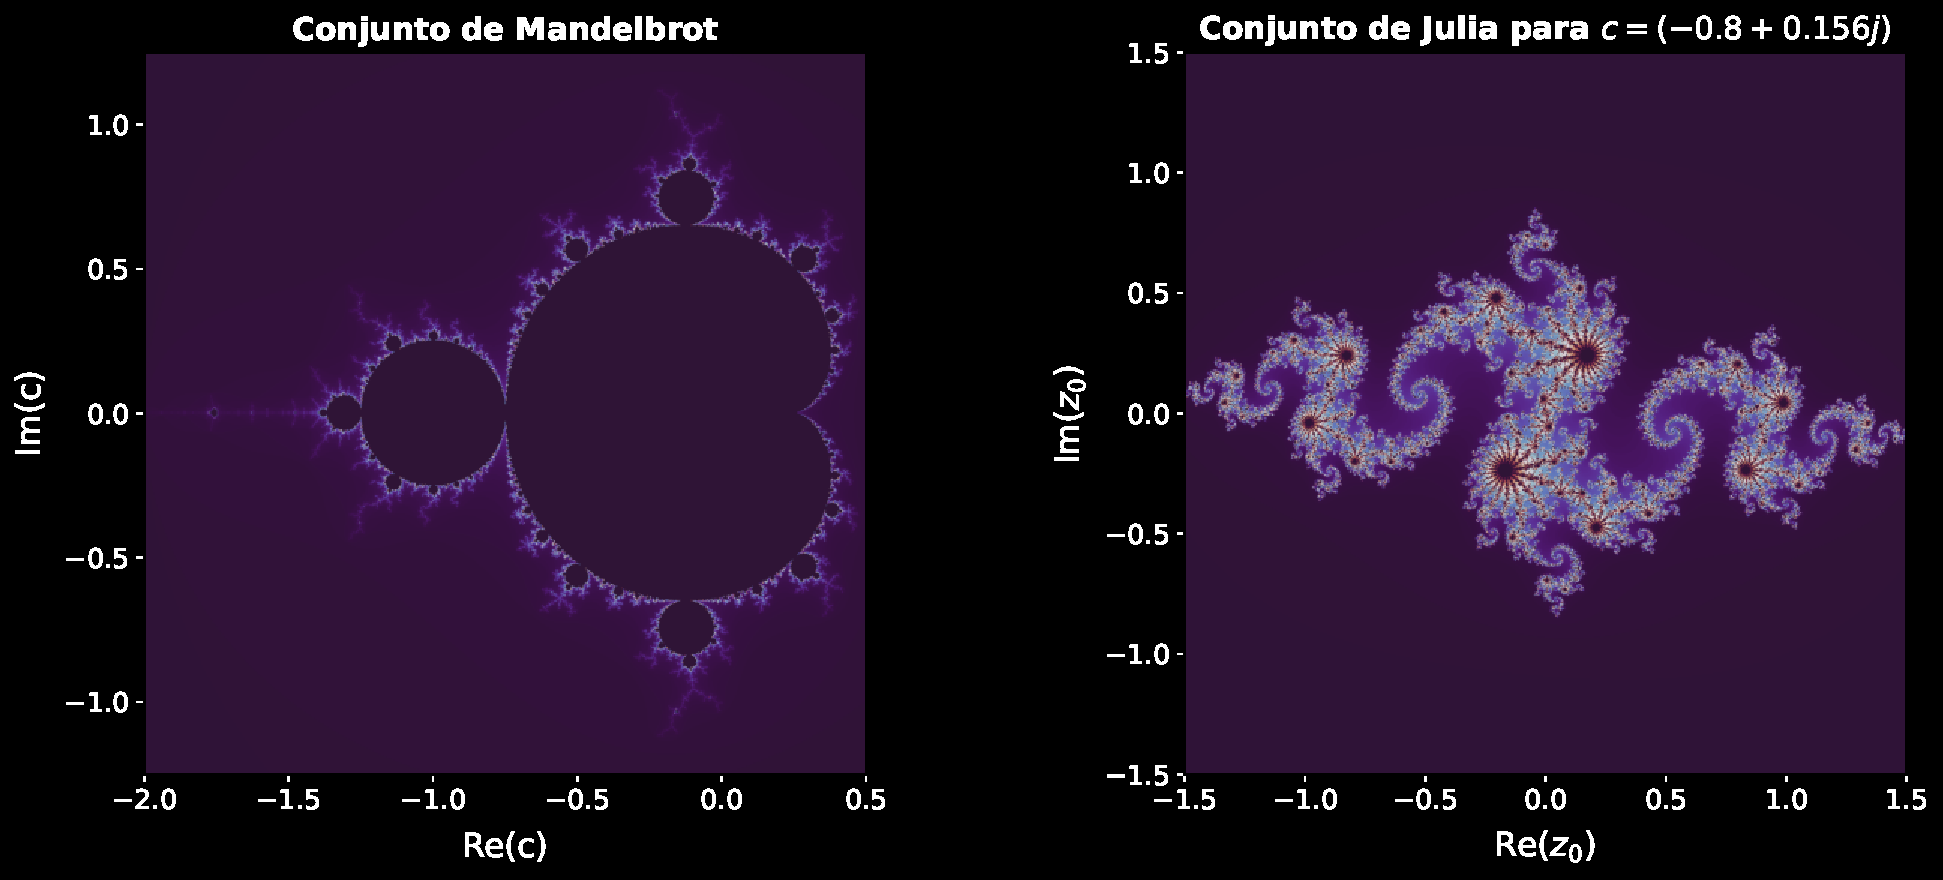
\includegraphics[width=0.95\textwidth]{julia_manderboot.pdf}
    \caption{Conjuntos de Julia y de Mandelbroot.}
\end{figure}
%

\begin{cajaflex}[\texttt{Resumen de las rutinas básicas utilizadas (Fractales e imshow)}]

$\blacklozenge$ Acceda a la documentación oficial \lstinline|matplotlib.pyplot.imshow| 
\href{https://matplotlib.org/stable/api/_as_gen/matplotlib.pyplot.imshow.html}{dando clic aquí}. 

\textcolor{teal!60!black}{\rule{\linewidth}{0.8pt}}

\vspace{0.1cm}

\subsubsection*{\textcolor{teal!70!black}{1. \texttt{y[:, None]} \mdseries{o} \texttt{y[:, np.newaxis]}}}
\begin{itemize}
    \item \textbf{Qué hace:} Inserta un nuevo eje dimensional al vector 1D de tamaño $(N,)$, transformándolo en una matriz columna de dimensiones $(N, 1)$.
    \item \textbf{Uso en broadcasting:} Permite que al operar un vector fila $x$ de tamaño $(M,)$ con $y_{[:, \text{None}]}$, NumPy expanda automáticamente la memoria y construya la cuadrícula bidimensional $C_{ij} = x_j + i y_i$ de dimensiones $(N, M)$ sin requerir bucles anidados lentos.
\end{itemize}

\subsubsection*{\textcolor{teal!70!black}{2. \texttt{np.zeros\_like(C, dtype=np.complex128)}}}
\begin{itemize}
    \item \textbf{Qué hace:} Reserva en memoria contigua una matriz de ceros con las dimensiones exactas de $C$, asignando explícitamente el tipo de dato complejo de doble precisión (128 bits: 64 bits para la parte real y 64 para la imaginaria).
    \item \textbf{Importancia numérica:} Evita truncamientos de coma flotante o excepciones de tipo al calcular potencias y productos con números imaginarios ($1j$).
\end{itemize}

\subsubsection*{\textcolor{teal!70!black}{3. \texttt{Z[mask]} \mdseries{y actualización mediante máscaras booleanas}}}
\begin{itemize}
    \item \textbf{Mecánica:} Filtra y evalúa la función iterativa cuadrática $z_{n+1} = z_n^2 + c$ exclusivamente sobre aquellos elementos donde \lstinline|mask == True| (los puntos cuya magnitud aún no supera la cota de escape).
    \item \textbf{Eficiencia computacional:} Reduce exponencialmente el costo temporal del bucle; a medida que los puntos exteriores escapan al infinito, la CPU deja de procesarlos y se enfoca únicamente en los bordes críticos del fractal.
\end{itemize}

\subsubsection*{\textcolor{teal!70!black}{4. \texttt{newly\_escaped = escaped \& mask} \mdseries{y} \texttt{mask \&= \textasciitilde escaped}}}
\begin{itemize}
    \item \textbf{Qué hace:} El operador bitwise AND (\lstinline|&|) aísla los puntos que violaron el radio de escape ($|z| > 2$) en el paso actual $i$, impidiendo sobreescribir las celdas de píxeles que ya habían escapado en pasos anteriores.
    \item \textbf{Actualización:} \lstinline|mask &= ~escaped| aplica una negación lógica (\lstinline|~|) que apaga a \lstinline|False| las posiciones divergentes para excluirlas en las siguientes iteraciones.
\end{itemize}

\subsubsection*{\textcolor{teal!70!black}{5. \texttt{ax.imshow(grid, extent, origin, cmap)}}}
\begin{itemize}
    \item \textbf{Entrada numérica:} Recibe una matriz bidimensional discreta donde cada valor representa la iteración de escape y le asigna un color continuo mediante la paleta \texttt{cmap}.
    \item \textbf{Parámetro \texttt{origin="lower"}:} Coloca el índice $y_{\min}$ en la parte inferior del eje vertical. Sin este parámetro, Matplotlib usa por defecto la convención matricial (\texttt{upper}), colocando la fila 0 arriba e invirtiendo el plano complejo de cabeza.
    \item \textbf{Parámetro \texttt{extent=[xmin, xmax, ymin, ymax]}:} Calibra el sistema de coordenadas de la figura, sustituyendo los índices discretos de píxeles $(0, 1, \dots, N)$ por las dimensiones físicas y matemáticas continuas del espacio complejo.
\end{itemize}
\end{cajaflex}

%--------------- problemas --------------------

\begin{problemas}[]
\begin{enumerate}[leftmargin=*]

\item \textbf{El conjunto de Mandelbrot}, nombrado en honor al matemático 
Benoit Mandelbrot, es un \textit{fractal}: un objeto geométrico 
infinitamente ramificado que contiene estructura dentro de estructura, 
sin importar cuánto nos acerquemos a mirarlo.

Se genera con una regla muy sencilla sobre números complejos:
\begin{equation}
    z_{n+1} = z_n^2 + c,
\end{equation}
donde $z$ y $c$ son números complejos. 

Para un valor fijo de $c$, comenzamos con $z_0 = 0$ y 
aplicamos la ecuación una y otra vez. 
Se dice que el punto $c$ pertenece al conjunto de Mandelbrot 
si el valor de $z$ no crece indefinidamente hacia el infinito. 
Matemáticamente se demuestra que si en algún momento 
la magnitud supera el valor 2 ($|z| > 2$), 
la secuencia se escapará al infinito con total certeza.

\paragraph{Instrucciones:}
\begin{enumerate}
    \item Defina una cuadrícula de puntos complejos $c = x + iy$ en la región 
    $-2 \le x \le 2$ y $-2 \le y \le 2$.
    \item Para cada punto de la cuadrícula, aplique la iteración $z_{n+1} = z_n^2 + c$ 
    comenzando con $z_0 = 0$ hasta un máximo de 100 pasos. 
    Si en algún paso intermedio $|z| > 2$, 
    detenga el cálculo y registre que ese punto escapó.
    \item Dibuje el resultado con un gráfico de densidad (\texttt{plt.imshow}). 
    Pinte de negro los puntos que quedaron atrapados dentro del conjunto y de color 
    claro los que escaparon.
    \item \textbf{Pista:} Empiece con una cuadrícula pequeña 
    (por ejemplo de $100 \times 100$) para probar que su código funcione rápido, 
    y luego aumente la resolución a $500 \times 500$ o más.
\end{enumerate}

\item \textbf{Los conjuntos de Julia} usan exactamente la misma fórmula que el ejercicio 
anterior ($z_{n+1} = z_n^2 + c$), pero con los papeles invertidos:
\begin{itemize}
    \item En lugar de variar $c$, dejamos una constante compleja $c$ fija para toda
     la simulación.
    \item Lo que cambia en cada píxel de la imagen es la condición inicial 
    $z_0 = x + iy$.
\end{itemize}

El conjunto de Julia reúne a todos los puntos iniciales $z_0$ que no se escapan a 
infinito bajo la iteración. 
Dependiendo del valor de $c$ que elijamos,
obtendremos figuras conectadas con patrones intrincados o figuras que se 
desmoronan en polvo.

\paragraph{Instrucciones:}
\begin{enumerate}
    \item Elija una constante compleja de prueba, 
    por ejemplo $c = -0.7 + 0.27015i$ o $c = -0.4 + 0.6i$.
    \item Construya una cuadrícula en el plano complejo para 
    $z_0 = x + iy$ en el intervalo $-1.5 \le x \le 1.5$ y $-1.2 \le y \le 1.2$.
    \item Itere la ecuación hasta 100 veces por cada punto. 
    Guarde en una matriz cuántas iteraciones tardó cada punto en superar la barrera $|z| > 2$.
    \item Muestre la imagen resultante con un mapa de color como 
    \texttt{"inferno"} o \texttt{"magma"}. Ensaye cambiando ligeramente el 
    valor de $c$ y observe cómo muta la figura.
\end{enumerate}

\item  \textbf{El juego del caos y el triángulo de Sierpinski} El juego del caos muestra cómo un proceso totalmente aleatorio puede construir una estructura geométrica perfecta sin necesidad de dibujar líneas directas:
\begin{enumerate}
    \item Dibujamos tres vértices fijos en el plano formando un triángulo equilátero:
    \begin{equation*}
        A = (0, 0), \quad B = (1, 0), \quad C = (0.5, \frac{\sqrt{3}}{2}).
    \end{equation*}
    \item Empezamos con un punto inicial cualquiera en el plano, por ejemplo $(0.5, 0.2)$.
    \item Lanzamos un dado de tres caras para elegir al azar uno de los tres vértices.
    \item Marcamos un nuevo punto exactamente en el punto medio entre la posición actual y el vértice seleccionado.
    \item Repetimos el proceso miles de veces, usando siempre el último punto marcado como punto de partida para el siguiente paso.
\end{enumerate}

\paragraph{Instrucciones:}
\begin{enumerate}
    \item Escriba un script que genere $50\,000$ puntos siguiendo estas reglas usando el generador de números aleatorios de NumPy.
    \item Descarte los primeros 100 puntos (son el transitorio mientras el caminante entra en la figura).
    \item Grafique todos los puntos acumulados con \texttt{plt.scatter} usando puntos muy pequeños (\texttt{s=0.1}). Verá formarse el triángulo de Sierpinski, con triángulos vacíos a todas las escalas.
\end{enumerate}

\item \textbf{Ramificación recursiva de un árbol} Muchos patrones en la naturaleza, como las ramas de los árboles o los vasos sanguíneos, crecen mediante una regla de división simple que se repite sobre sí misma a escalas cada vez más reducidas.

Podemos modelar un árbol básico con los siguientes pasos:
\begin{enumerate}
    \item Trazamos un tronco vertical desde la base con una longitud $L$.
    \item Al final del tronco, nacen dos ramas hijas: una desviada hacia la izquierda (ángulo $+\theta$) y otra hacia la derecha (ángulo $-\theta$).
    \item Cada rama hija mide un porcentaje de la rama padre (por ejemplo, el 70\%: $L_{\text{nueva}} = 0.7 L$).
    \item En la punta de cada rama hija, repetimos la división de forma sucesiva hasta llegar a un límite de ramificaciones (por ejemplo, 8 o 9 niveles).
\end{enumerate}

\paragraph{Instrucciones:}
\begin{enumerate}
    \item Escriba una función recursiva corta que dibuje este árbol usando segmentos con \texttt{plt.plot}.
    \item Pruebe con ángulos de apertura de $20^\circ$, $30^\circ$ y $45^\circ$, y note cómo cambia la silueta.
    \item \textbf{Opcional:} Añada una variación aleatoria leve en cada bifurcación (en el ángulo y en la longitud) para transformar el patrón geométrico rígido en un árbol de apariencia natural.
\end{enumerate}

\item \textbf{El mapa logístico y el caos determinista} En 1976, Robert May popularizó una ecuación elemental para modelar cómo cambia año a año el tamaño de una población de insectos en un cultivo:
\begin{equation}
    x_{n+1} = r \, x_n (1 - x_n).
\end{equation}
Aquí, $x_n$ es la población normalizada entre 0 (extinción) y 1 (capacidad máxima del entorno), y $r$ es la tasa de crecimiento (entre 0 y 4). El término $x_n$ favorece los nacimientos, mientras que $(1 - x_n)$ simula la limitación por alimento y espacio.

Aunque la fórmula no contiene azar, su comportamiento a largo plazo cambia radicalmente según el valor de $r$:
\begin{itemize}
    \item Para valores pequeños de $r$, la población se estabiliza en un valor fijo.
    \item Al subir $r$, la población empieza a oscilar entre dos valores fijos, luego cuatro, ocho...
    \item Para $r > 3.57$, el sistema entra en un comportamiento caótico: la población nunca se repite y varía de forma impredecible.
\end{itemize}

\paragraph{Instrucciones:}
\begin{enumerate}
    \item Tome una secuencia de valores para $r$ entre 2.5 y 4.0 con pasos pequeños (por ejemplo, 1000 valores).
    \item Para cada $r$, inicie con una población arbitraria (como $x_0 = 0.5$) e itere la ecuación 300 veces sin guardar nada, para permitir que el sistema olvide la condición inicial.
    \item Itere 100 veces adicionales y guarde los valores resultantes de $x$.
    \item Grafique los puntos $(r, x)$ usando puntos diminutos (\texttt{plt.plot(r, x, ',k', alpha=0.25)}). Obtendrá el famoso diagrama de bifurcación con la cascada hacia el caos.
\end{enumerate}

\item \textbf{Decaimiento radiactivo con Monte Carlo} El decaimiento radiactivo es un proceso inherentemente probabilístico: es imposible saber cuándo decaerá un núcleo atómico individual, pero sabemos que en cada segundo tiene una probabilidad fija $p$ de transformarse.

Podemos simular este fenómeno átomo por átomo:
\begin{quote}
    \itshape
    En cada segundo, revisamos cada uno de los átomos activos de la muestra y generamos un número aleatorio uniforme entre 0 y 1. Si el número obtenido es menor que $p$, el átomo decae y desaparece de la cuenta; si no, sobrevive al siguiente segundo.
\end{quote}

\paragraph{Instrucciones:}
\begin{enumerate}
    \item Inicie con una muestra de $N_0 = 5000$ átomos y una probabilidad de decaimiento por paso de $p = 0.03$.
    \item Simule el proceso durante 150 pasos de tiempo. En cada paso, use el generador de números aleatorios para determinar cuántos átomos sobreviven y actualice el total.
    \item Grafique el número de átomos sobrevivientes en función del tiempo.
    \item En la misma gráfica, compare sus puntos de simulación con la curva teórica exponencial $N(t) = N_0 e^{-\lambda t}$, donde $\lambda = p$.
    \item Encuentre visual o numéricamente el tiempo que tarda la muestra en reducirse a la mitad ($N_0 / 2$) y verifique si coincide con la vida media teórica $t_{1/2} = \frac{\ln(2)}{p}$.
\end{enumerate}

\end{enumerate}
\end{problemas}




\end{document}

